\chapter{Solov'ev Analytical Tokamak Equilibrium}
Here, the analytical Solov'ev Tokamak equilibrium
presented in Ref.~\cite{hirshman_whitson_1983}
is investigated and converted to VMEC inputs.
%
This set of notes is based on the investigations
on this topic by J. D. Hanson (Auburn University),
which were distributed as Mathematica Notebooks,
and TeX-ed here for further work.

\section{Setup}

\subsection{Information Survey from Sec. VI.}
Here, we collect all information
related to the Solov'ev equilibrium
available in the section ``I.~Introduction''
of the original article.

\begin{itemize}

\item
In the axisymmetric case, can integrate $F_\beta = 0$ to yield:
\begin{equation}
 B_\zeta = F(\rho) \label{eqn:bsubv_f}
\end{equation}

\item
Some metric elements vanish:
\begin{equation}
 g_{\theta \zeta} = g_{\rho \zeta} = 0
\end{equation}

\item
axisymmetry implies:
\begin{equation}
 \frac{\partial \lambda}{\partial \zeta} = 0
\end{equation}

\item
Contravariant magnetic field component:
\begin{equation}
 B^\zeta = \frac{B_\zeta}{g_{\zeta \zeta}}
\end{equation}
with
\begin{equation}
 g_{\zeta \zeta} = R^2
\end{equation}
where $R$ is the major radius

\item
now find the inverse Grad-Shafranov equation:
\begin{equation}
 F_\rho = \frac{\chi'}{\mu_0 \sqrt{g}}
 \left[
   \frac{\partial}{\partial \rho  } \left( \frac{\chi' g_{\theta \theta}}{\sqrt{g}} \right) -
   \frac{\partial}{\partial \theta} \left( \frac{\chi' g_{\rho   \theta}}{\sqrt{g}} \right)
 \right]
 + \frac{F F'}{\mu_0 R^2}
 + p'
\end{equation}

\item
We can also write Eqn.~\ref{eqn:bsubv_f} as:
\begin{equation}
 F(\rho) = \frac{\phi' R^2}{\sqrt{g}} \left( 1 + \frac{\partial \lambda}{\partial \theta} \right)
\end{equation}

\item
This yields
\begin{equation}
 \phi'(\rho) = \langle \frac{\sqrt{g}}{R^2} \rangle F(\rho)
\end{equation}

\item
and
\begin{equation}
 \frac{\partial \lambda}{\partial \theta}
 = \frac{\sqrt{g} / R^2}{\langle \sqrt{g} / R^2 \rangle} - 1
\end{equation}
where the $\langle . \rangle$ denotes a normalized $\theta$ average.

\end{itemize}


\subsection{Information Survey from Sec. VI.}
Here, we collect all information
related to the Solov'ev equilibrium
available in the section ``VI.~Moment Analysis of Solov'ev Equilibrium''
of the original article.

\begin{itemize}

\item
The magnetic field is represented as
\begin{equation}
 \mathbf{B} = \chi' \nabla \zeta \times \nabla \rho + F(\rho) \nabla \zeta \, .
\end{equation}

\item
A solution to the axisymmetric Grad-Shafranov equation,
with the above representation of the magnetic field, is:
\begin{equation}
 \rho^2 = \frac{\beta_1}{\chi_0^2}
 \left[
   Z^2 R_0^2 + \left( \frac{\beta_0}{8 \beta_1} \right) \left( R^2 - R_m^2 \right)^2
 \right]
\end{equation}

\item
where
\begin{equation}
 \chi' = 2 \rho \chi_0 \label{eqn:chip}
\end{equation}

\item
$\rho^2$ is the normalized poloidal flux $0 \leq \rho \leq 1$

\item
The pressure profile is
\begin{equation}
 p(\rho) = \beta_0 \left( 1 - \rho^2 \right)
\end{equation}

\item
The current flux function~$F$ is
\begin{equation}
 F^2 = R_0^2 \left( 1 - 4 \beta_1 \rho^2 \right)
\end{equation}

\item
The toroidal field is normalized to unity,
if $R_0$ is identified with the mean major radius;
this says something about \texttt{phiedge}.

\item
Note that $R = R_m$ is the magnetic axis,
which is determined by the boundary curve $\rho = 1$.
This could either be a typo (the axis is at $\rho = 0$),
or it is meant to say that the boundary geometry determines the magnetic axis position,
and the magnetic axis geometry is not something the user can freely choose.

\item
The spectral analysis is trivial in terms of the variables
$u = R^2$ and $Z$, yielding:
\begin{align}
 u =
 R^2 =&\, R_m^2 - \chi_0 \sqrt{\frac{8}{\beta_0}} \rho \cos(\theta) \\
 Z   =&\, \frac{\chi_0}{R_0} \frac{1}{\sqrt{\beta_1}} \rho \sin(\theta)
\end{align}

\item
Here, $\theta$ is a geometric angle
yielding a rapidly converging Fourier expansion for $R$ and $Z$,
which is not equal to the magnetic angle $\theta^*$,
in which magnetic field lines are straigt.

\item
The Jacobian is
\begin{equation}
 \sqrt{g} = \frac{\chi_0^2}{R_0} \sqrt{\frac{2}{\beta_0 \beta_1}} \rho
\end{equation}

\item
It is easy to evaluate $\lambda$ explicitly:
\begin{equation}
 \lambda_\theta = \frac{\sqrt{1 - a^2}}{1 - a \cos(\theta)} - 1
\end{equation}
where
\begin{equation}
 a(\rho) = \frac{\chi_0}{R_m^2} \sqrt{\frac{8}{\beta_0}} \rho < 1 \label{eqn:def_a}
\end{equation}

\item
Thus:
\begin{equation}
 \lambda = \sum_{m = 1} \hat{\lambda}_m \sin(m \theta)
\end{equation}
with
\begin{equation}
 \hat{\lambda}_m = \frac{2}{m} \left[ \frac{1}{a} \left( 1 - \sqrt{1 - a^2} \right) \right]^m
\end{equation}

% TODO: What is the correct asymptotic behaviour towards the magnetic axis?
%       It seems that $a$ goes to zero as $\rho$ goes to zero,
%       and $\hat{\lambda}_m$ blows up because it depends on $1/a$?

\item
Note that for $a^2 < 1$, $\hat{\lambda}_m$ decays exponentially with $m$.

\item
The magnetic flux profile is found to be
\begin{equation}
 \frac{\phi'}{\chi'} \equiv q(\rho)
 = \frac{\chi_0}{R_m^2}
 \sqrt{
   \frac{1}{2 \beta_0 \beta_1} \left( \frac{1 - 4 \beta_1 \rho^2}{1 - a^2} \right)
 }
\end{equation}

\end{itemize}


\subsection{Information Survey from Sec. VI.}
Here, we collect all information
related to the Solov'ev equilibrium
available in the section ``IX. Numerical Examples''
of the original article.

\begin{itemize}

\item
The value of $R_0(0)$ should be $4$.

\item
The caption of Figure 2 lists
a few more parameters:

\item
$R$ of the boundary geometry:
\begin{equation}
 \left(\frac{R}{4}\right)^2 = 1 - \frac{1}{2} \rho \cos(\theta)
\end{equation}

\item
$Z$ of the boundary geometry:
\begin{equation}
 Z = \frac{\sqrt{10}}{2} {\color{red} \rho} \sin(\theta)
\end{equation}
Note that the $\rho$ was probably forgotten in the article.

\item
The pressure profile is:
\begin{equation}
 p(\rho) = \frac{1}{8} (1 - \rho^2)
\end{equation}

\item
The poloidal flux profile is:
\begin{equation}
 \chi = \rho^2
\end{equation}

\end{itemize}

\section{Derived Quantities}

\subsection{Rotational Transform Profile}
One can simply compute $\iota = 1 / q$ as follows:
\begin{align}
 \iota(\rho) = \frac{1}{q(\rho)}
 =&\, \frac{1}{
  \frac{\chi_0}{R_m^2}
 \sqrt{
   \frac{1}{2 \beta_0 \beta_1} \left( \frac{1 - 4 \beta_1 \rho^2}{1 - a^2} \right)
 }
           } \nonumber \\
 =&\,
 \frac{R_m^2}{\chi_0}
 \sqrt{2 \beta_0 \beta_1 \left( \frac{1 - a^2}{1 - 4 \beta_1 \rho^2} \right)}
\end{align}
and with $a$ from Eqn.~\ref{eqn:def_a} we find:
\begin{align}
 \iota(\rho)
 =&\, \frac{R_m^2}{\chi_0} \sqrt{2 \beta_0 \beta_1 \left( \frac{1 - \left[ \frac{\chi_0}{R_m^2} \sqrt{\frac{8}{\beta_0}} \rho \right]^2}{1 - 4 \beta_1 \rho^2} \right)} \nonumber \\
 =&\, \frac{R_m^2}{\chi_0} \sqrt{2 \beta_0 \beta_1 \left( \frac{1 - \frac{\chi_0^2}{R_m^4} \frac{8}{\beta_0} \rho^2}{1 - 4 \beta_1 \rho^2} \right)}
\end{align}

\subsection{Toroidal Flux}
VMEC profiles are specified in terms of the toroidal magnetic flux.
We know:
\begin{equation}
 \iota = \frac{\chi'}{\phi'} \equiv \frac{\partial \chi}{\partial \rho} / \frac{\partial \phi}{\partial \rho}
\end{equation}
for some radial coordinate~$\rho$.
This can be reformulated as:
\begin{equation}
 \frac{\partial \phi}{\partial \rho} = \frac{1}{\iota} \frac{\partial \chi}{\partial \rho}
\end{equation}
and we can integrate radially to get the toroidal flux profile:
\begin{equation}
 \phi(\rho) = \int\limits_{0}^{\rho} \frac{1}{\iota} \frac{\partial \chi}{\partial \rho'} \,\mathrm{d}\rho'
\end{equation}
assuming that $\phi(0) = 0$ at the magnetic axis.
We know $\chi'$ already from Eqn.~\ref{eqn:chip}:
\begin{equation}
 \phi(\rho)
 = \int\limits_{0}^{\rho} \frac{2 \rho' \chi_0}{\iota} \,\mathrm{d}\rho'
 = \int\limits_{0}^{\rho} 2 \rho' \chi_0 q(\rho') \,\mathrm{d}\rho'
\end{equation}
and using the expression for the safety factor, we get:
\begin{align}
 \phi(\rho) =&\, 2 \chi_0 \int\limits_{0}^{\rho}
 \rho'
 \frac{\chi_0}{R_m^2}
 \sqrt{
   \frac{1}{2 \beta_0 \beta_1} \left( \frac{1 - 4 \beta_1 {\rho'}^2}{1 - a^2(\rho')} \right)
 }
 \,\mathrm{d}\rho' \nonumber \\
 =&\, 2 \frac{\chi_0^2}{R_m^2} \sqrt{\frac{1}{2 \beta_0 \beta_1}}
   \int\limits_{0}^{\rho}
     \rho'
     \sqrt{\frac{1 - 4 \beta_1 {\rho'}^2}{1 - \beta_2^2 {\rho'}^2}}
     \,\mathrm{d}\rho'
\end{align}
The abstract integral used here can be solved by Wolfram Alpha:
\begin{align}
 \int x \sqrt{\frac{1 - a x^2}{1 - b x^2}} \,\mathrm{d}x
 =&\,
 \frac{1}{2 a b^{3/2} (a x^2 - 1)}
 \sqrt{b - a}
 \sqrt{\frac{a x^2 - 1}{b x^2 - 1}}
 \sqrt{\frac{a - a b x^2}{a - b}}
 \Biggl[
 \nonumber \\
~& \phantom{+}~ \sqrt{b}
   \sqrt{b - a}
   (a x^2 - 1)
   \sqrt{\frac{a (b x^2 - 1)}{b - a}}
   \nonumber \\
~& + (a - b)
   \sqrt{a x^2 - 1}
   \,\mathrm{sinh}^{-1} \left(
     \frac{\sqrt{b} \sqrt{a x^2 - 1}}{\sqrt{b - a}}
   \right)
 \Biggr]
\end{align}
A direct inverse of this function is not obvious,
which is why finding the value of $\rho$ for a given value of $\phi$
will be done numerically for the time being.

One could also think about using VMEC in \texttt{lRFP} mode,
where the poloidal flux is constrained and used as radial variable.

\subsection{Jacobian}

The VMEC-like Jacobian is given by:
\begin{equation}
 \sqrt{g} = R \tau
\end{equation}
with
\begin{align}
 \tau = R_\theta Z_s - R_s Z_\theta \, .
\end{align}

The radial derivatives with respect to $s$ are computed as follows.
The analytical model uses $\rho$ as the radial coordinate.
Since $\iota$ is constant, we have $\rho = \sqrt{s}$
with the normalized toroidal flux $s = \phi / \phi_\textrm{LCFS}$.
This implies for the radial derivatives:
\begin{align}
 R_s = \frac{\mathrm{d}R}{\mathrm{d}s}
 = \frac{\mathrm{d}R}{\mathrm{d}\rho} \frac{\mathrm{d}\rho}{\mathrm{d}s}
 = R_\rho \frac{\mathrm{d}\rho}{\mathrm{d}s}
\end{align}
and with the definition of $\rho$ we have
\begin{align}
 \frac{\mathrm{d}\rho}{\mathrm{d}s}
 = \frac{\partial}{\partial s} \left( \sqrt{s} \right)
 = \frac{1}{2 \sqrt{s}} = \frac{1}{2 \rho}
\end{align}
It thus follows:
\begin{align}
 R_s = R_\rho \frac{1}{2 \rho}
\end{align}

First order finite-differences are used for the radial derivatives:
\begin{align}
 R_s(s_{j+0.5}, \theta_l) =&\,
   \frac{R(s_{j+1}, \theta_l) - R(s_{j}, \theta_l)}{s_{j+1} - s_{j}}
\end{align}

Linear interpolation is used for the poloidal derivatives:
\begin{align}
 R_\theta(s_{j+0.5}, \theta_l) =&\,
   \frac{R_\theta(s_{j+1}, \theta_l) + R_\theta(s_{j}, \theta_l)}{2}
\end{align}


\subsection{Fourier Representation of the Boundary}

The expressions for the Fourier coefficients of the flux surface geometry are:
\begin{align}
 \hat{R}^\textrm{cos}_m(\rho) =&\,
   \frac{2 - \delta_{m,0}}{2 \pi}
   \int_{0}^{2 \pi}
     R(\rho, \theta) \cos(m \theta) \,\mathrm{d}\theta \\
 \hat{Z}^\textrm{sin}_m(\rho) =&\,
   \frac{2 - \delta_{m,0}}{2 \pi}
   \int_{0}^{2 \pi}
     Z(\rho, \theta) \sin(m \theta) \,\mathrm{d}\theta
\end{align}
Note that $Z$ only has a single Fourier coefficient:
\begin{align}
 Z =&\, \frac{\chi_0}{R_0} \frac{1}{\sqrt{\beta_1}} \rho \sin(\theta) \\
 \Rightarrow
 \hat{Z}^\textrm{sin}_1(\rho) =&\, \frac{\chi_0}{R_0} \frac{1}{\sqrt{\beta_1}} \rho
\end{align}
However, $R$ has more Fourier coefficients.
Note that:
\begin{align}
  R^2 =&\, R_m^2 - \chi_0 \sqrt{\frac{8}{\beta_0}} \cos(\theta) \\
  \Leftrightarrow
  \left( \frac{R}{R_m} \right)^2
    =&\, 1 - \underbrace{\frac{\chi_0}{R_m^2} \sqrt{\frac{8}{\beta_0}}}_{\equiv \beta_2} \rho \cos(\theta)
\end{align}
and hence
\begin{align}
 \frac{R}{R_m} = \sqrt{ 1 - \beta_2 \rho \cos(\theta) }
\end{align}
For $m=0$, it thus follows:
\begin{align}
 \hat{R}^\textrm{cos}_0(\rho)
%  =&\,
%    \frac{1}{2 \pi}
%    \int_{0}^{2 \pi}
%      R(\rho, \theta)
%      \,\mathrm{d}\theta \\
 =&\,
   \frac{R_m}{2 \pi}
   \int_{0}^{2 \pi}
     \sqrt{ 1 - \beta_2 \rho \cos(\theta) }
     \,\mathrm{d}\theta
\end{align}
This is a complete elliptic integral
and can therefore be evaluated analytically.
% as:
% \begin{align}
%  \hat{R}^\textrm{cos}_0(\rho)
%  =&\,
%  TODO
% \end{align}
For $m>0$, we have:
\begin{align}
 \hat{R}^\textrm{cos}_m(\rho)
 =&\,
   \frac{R_m}{\pi}
   \int_{0}^{2 \pi}
     \sqrt{ 1 - \beta_2 \rho \cos(\theta) }
     \cos(m \theta)
     \,\mathrm{d}\theta \\
\end{align}

Adaptive arbitrary-precision quadrature was used to compute the Fourier coefficients
of $R$ for a number of poloidal modes.
\begin{figure}[h]
 \centering
 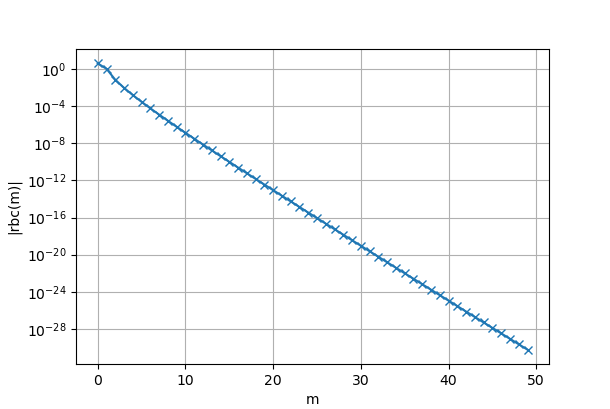
\includegraphics[width=0.5\textwidth]{img/solovev/rbc_decay.png}
 \caption{Decay of the boundary geometry coefficients for $R$ with poloidal mode number $m$.}
\end{figure}

% \subsection{Scan of $\beta_1$}
% The value of $\beta_1$ is $1/16$ in case of a flat profile of $\iota$.
% This is assumed to be case that is published in the 1983 article.
% This value has been scanned over the values $1/32$ (blue), $1/16$ (orange) and $1/8$ (green) in the following plots.

% \begin{figure}[h]
%  \centering
%  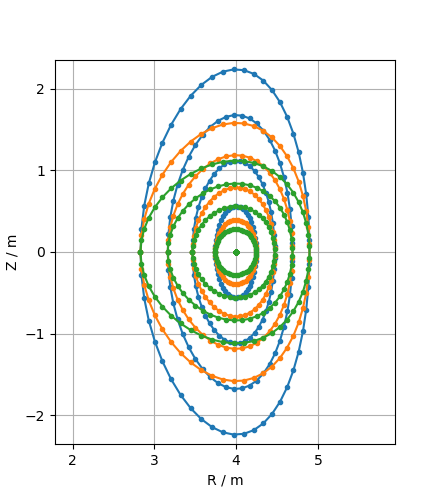
\includegraphics[width=0.5\textwidth]{img/solovev/boundary_shapes.png}
%  \caption{Boundary and inner flux surfaces shapes.
%           $\beta_1 = 1/32$ (blue), $1/16$ (orange) and $1/8$ (green).}
% \end{figure}


% \begin{figure}[h]
%  \centering
%  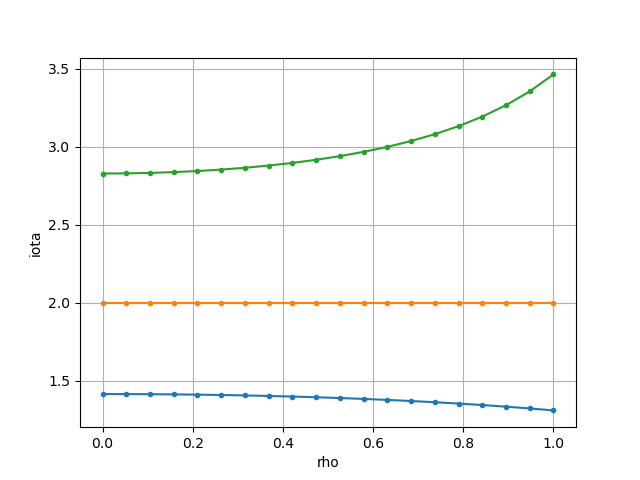
\includegraphics[width=0.5\textwidth]{img/solovev/iota_profiles.png}
%  \caption{Rotational transform profile.
%           $\beta_1 = 1/32$ (blue), $1/16$ (orange) and $1/8$ (green).}
% \end{figure}

% \begin{figure}[h]
%  \centering
%  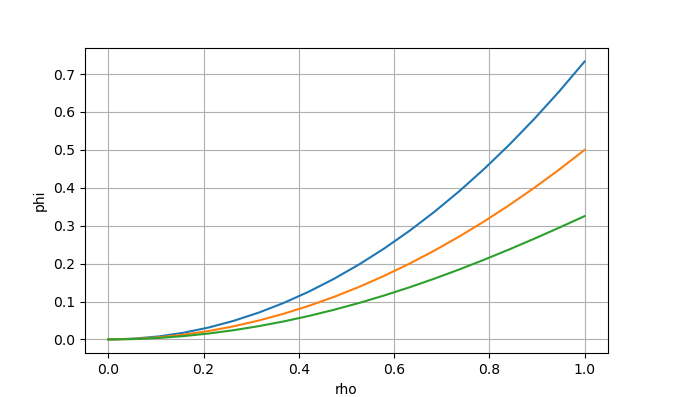
\includegraphics[width=0.5\textwidth]{img/solovev/phi_profiles.png}
%  \caption{Toroidal flux function $\phi$ profile.
%           $\beta_1 = 1/32$ (blue), $1/16$ (orange) and $1/8$ (green).}
% \end{figure}



% \begin{figure}[h]
%  \centering
%  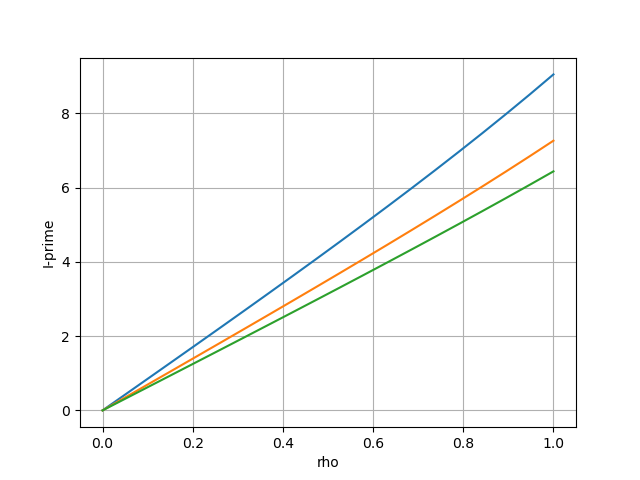
\includegraphics[width=0.5\textwidth]{img/solovev/iprime_profiles.png}
%  \caption{Profile of radial derivative of enclosed toroidal current (I-prime).
%           $\beta_1 = 1/32$ (blue), $1/16$ (orange) and $1/8$ (green).}
% \end{figure}

